\documentclass[11pt,a4paper]{article}
\usepackage[margin=24mm,headheight=14pt]{geometry}
\usepackage{fontspec}
\setmainfont{TeXGyreTermes}
\setsansfont{TeXGyreHeros}
\usepackage{unicode-math}
\setmathfont{STIX Math}
\usepackage{microtype}
\usepackage{graphicx,booktabs,array,tabularx,caption,float,needspace}
\usepackage{amsmath,mathtools}
\usepackage{fancyhdr,lastpage}
\usepackage[unicode,colorlinks=true,linkcolor=black,urlcolor=black]{hyperref}
\usepackage{enumitem}
\usepackage{xcolor}
\definecolor{ink}{HTML}{202B37}
\definecolor{slate}{HTML}{536271}
\definecolor{rule}{HTML}{ABB4BF}
\color{ink}
\setlength{\parindent}{0pt}
\setlength{\parskip}{6pt}
\linespread{1.10}
\setlist[itemize]{leftmargin=1.5em,itemsep=2pt,topsep=2pt}
\captionsetup{font=small,labelfont=bf,justification=centering,skip=5pt}
\pagestyle{fancy}
\fancyhf{}
\fancyhead[L]{\footnotesize\sffamily INDUSTRIAL PROCESS CONTROL}
\fancyhead[R]{\footnotesize\sffamily TECHNICAL REPORT}
\renewcommand{\headrulewidth}{.35pt}
\fancyfoot[C]{\footnotesize\thepage\ / \pageref{LastPage}}
\newcommand{\Fig}[3][.83\linewidth]{\begin{figure}[H]\centering\includegraphics[width=#1,keepaspectratio]{#2}\caption{#3}\end{figure}}
\newcommand{\sechead}[1]{\needspace{5\baselineskip}\section{#1}}
\begin{document}
\thispagestyle{empty}
\vspace*{28mm}
{\sffamily\large\color{slate} CONTROL ENGINEERING \quad / \quad RESEARCH-BASED PROJECT REPORT\par}
\vspace{8mm}
{\fontsize{28}{33}\selectfont\bfseries Industrial Process Control\par}
\vspace{3mm}
{\fontsize{18}{23}\selectfont System Identification, PID Tuning, and Smith Prediction\par}
\vspace{11mm}
\noindent\rule{\linewidth}{.8pt}
\vspace{8mm}
{\large\itshape Modeling and control of a delayed fourth-order process using MATLAB and Simulink\par}
\vspace{10mm}
\begin{tabularx}{\linewidth}{@{}>{\bfseries}p{39mm}X@{}}
Research focus & Reduced-order identification, relay feedback, PID tuning, delay compensation\\[5pt]
Plant & Fourth-order rational transfer function with 2.5-s transport delay\\[5pt]
Evidence & Original MATLAB/Simulink sources; recorded simulation figures; independent model-comparison calculations\\
\end{tabularx}
\vfill
{\footnotesize\color{slate} Technical portfolio edition. Calculated results and archived simulation evidence are differentiated throughout. No additional hardware measurements are claimed.\par}
\clearpage
\section*{Abstract}
A fourth-order process with a 2.5-second transport delay is investigated through low-order system identification, relay-feedback experiments, PID tuning, and Smith-predictor simulation. First-order-plus-dead-time (FOPDT) and second-order-plus-dead-time (SOPDT) approximations are compared with the reference process using unit-step responses and root-mean-square error (RMSE). The identified model parameters are taken from the original analysis, while numerical response comparisons have been recomputed independently. Historical Simulink figures document controller tuning and predictor experiments; these are interpreted as experimental evidence rather than an independently rerun performance benchmark. The report separates demonstrated results, analytical interpretation, and remaining validation needs.

\noindent\textbf{Keywords:} process control; system identification; dead time; FOPDT; SOPDT; relay feedback; PID control; Smith predictor.

\sechead{Process Definition}
The plant in the supplied project is
\begin{equation}
G(s)=\frac{1000e^{-2.5s}}{s^{4}+126s^{3}+2725s^{2}+12600s+1000}.
\label{eq:plant}
\end{equation}
Its rational factor describes the process dynamics, and $e^{-2.5s}$ introduces a pure transport delay. The exact direct-current (DC) gain is
\begin{equation}
K_{\mathrm{DC}}=\lim_{s\to0}G(s)=\frac{1000}{1000}=1.
\end{equation}
The original response-based estimate of approximately $0.990211$ is not the exact mathematical DC gain. This distinction matters when interpreting identified gain parameters or steady-state error.

\sechead{Reduced-Order Identification}
Two approximate structures are considered:
\begin{align}
G_{\mathrm{FOPDT}}(s)&=\frac{K_3e^{-L_3s}}{T_3s+1},\\
G_{\mathrm{SOPDT}}(s)&=\frac{K_4e^{-L_4s}}{(T_1s+1)(T_2s+1)}.
\end{align}
These retain a transport-delay term while replacing the fourth-order denominator by a first- or second-order dynamic model. Table~\ref{tab:identified} reproduces the parameters recorded in the original project. They were not re-optimized when preparing this report.
\begin{table}[H]\centering
\caption{Recorded reduced-order identification parameters.}\label{tab:identified}
\begin{tabular}{@{}lrr@{}}\toprule
Parameter & FOPDT & SOPDT\\\midrule
Gain, $K$ & 0.990211 & 0.990211\\
Delay, $L$ (s) & 2.698647 & 2.698647\\
Dominant time constant (s) & 12.201353 & 12.128868\\
Second time constant (s) & --- & 0.063750\\\bottomrule
\end{tabular}
\end{table}

\subsection{Step-response comparison}
The reported models and the reference process were compared with a unit-step input over $0\le t\le60$~s and a sample interval of $\Delta t=0.02$~s. For reference values $y_i$ and approximate values $\hat y_i$,
\begin{equation}
\mathrm{RMSE}=\sqrt{\frac{1}{N}\sum_{i=1}^{N}(y_i-\hat y_i)^2}.
\label{eq:rmse}
\end{equation}
\Fig[.89\linewidth]{images/model_comparison.png}{Recomputed unit-step responses of the reference fourth-order process and the reported reduced-order models.}
\begin{table}[H]\centering
\caption{Independent sampled-response comparison for the specified window.}\label{tab:rmse}
\begin{tabular}{@{}lr@{}}\toprule Model & RMSE\\\midrule
FOPDT (three-parameter) & 0.005663\\
SOPDT (four-parameter) & 0.005250\\\bottomrule\end{tabular}
\end{table}
For this sampled step response, the SOPDT model has a slightly lower RMSE. The result is specific to the stated models, input, sample spacing, and evaluation horizon; it is not proof of superior performance for all possible operating conditions.
\Fig[.88\linewidth]{images/model_errors.png}{Signed residuals of the reduced-order step responses relative to the original delayed process.}

\sechead{Relay Feedback and PID Tuning}
The submitted experiment uses relay feedback to elicit oscillatory behavior and inform an ultimate-point-based tuning procedure. The associated relay signal and recorded process response are presented in Figure~\ref{fig:relay}; they have not been re-executed as part of this documentation revision.
\begin{figure}[H]\centering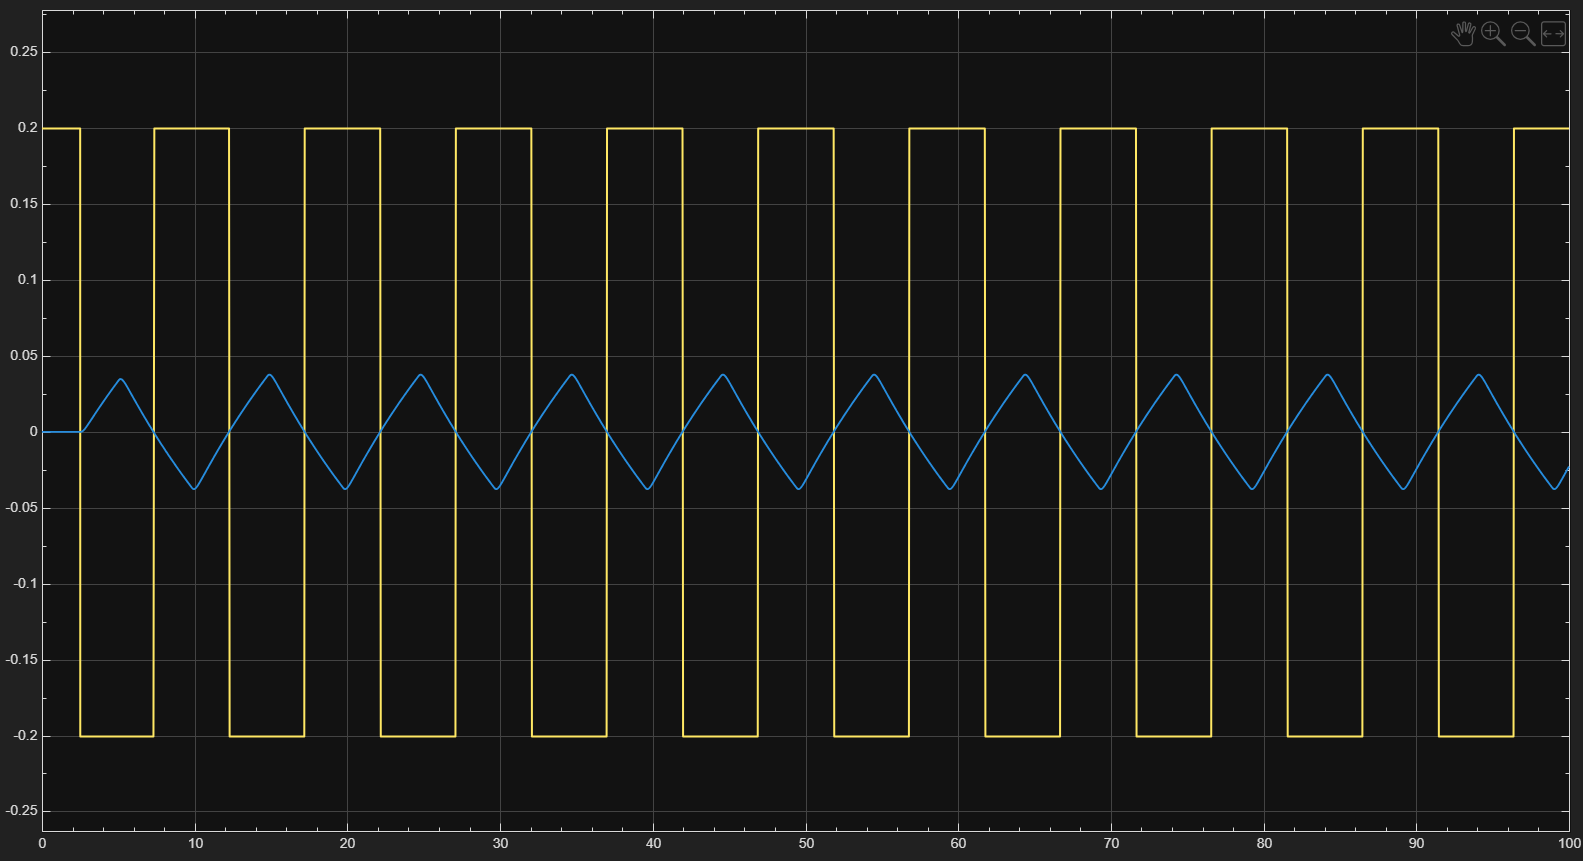
\includegraphics[width=.85\linewidth]{images/relay_feedback.png}\caption{Relay-feedback experiment: recorded switching behavior and process response from the original simulation study.}\label{fig:relay}\end{figure}
The project investigates time-domain and frequency-domain Ziegler--Nichols tuning, a generalized Ziegler--Nichols variant, and a $\lambda$-based design. The ideal continuous-time PID law may be written as
\begin{equation}
C(s)=K_p+\frac{K_i}{s}+K_ds.
\end{equation}
A tuning rule produces an initial controller; satisfactory performance still depends on the chosen trade-offs, plant delay, model fidelity, and any implementation constraints. The archived responses illustrate sensitivity to parameter choices rather than a universally optimal set of gains.
\Fig[.79\linewidth]{images/pid_time_domain.png}{Recorded PID step-response example from the original controller-tuning study.}
\Fig[.79\linewidth]{images/lambda_tuning.png}{Recorded simulation response for a $\lambda$-based PID tuning experiment.}

\sechead{Smith-Predictor Investigation}
A Smith predictor uses a process model to account for dead time in the feedback structure. Under ideal model matching, separating nominal delay-free dynamics from the delayed plant output can improve the feedback design problem. In practice, the result depends strongly on the fidelity of gain, time constants, and delay estimates.
\Fig[.80\linewidth]{images/smith_structure.png}{Smith-predictor arrangement reproduced from the documented Simulink study.}
The project compares predictor experiments under different assumptions about model knowledge, including the identified FOPDT model. Figure~\ref{fig:smithcompare} preserves the reported behavior as historical simulation evidence. The numerical solver settings and full suite of repeated trials were not independently audited for this edition.
\begin{figure}[H]\centering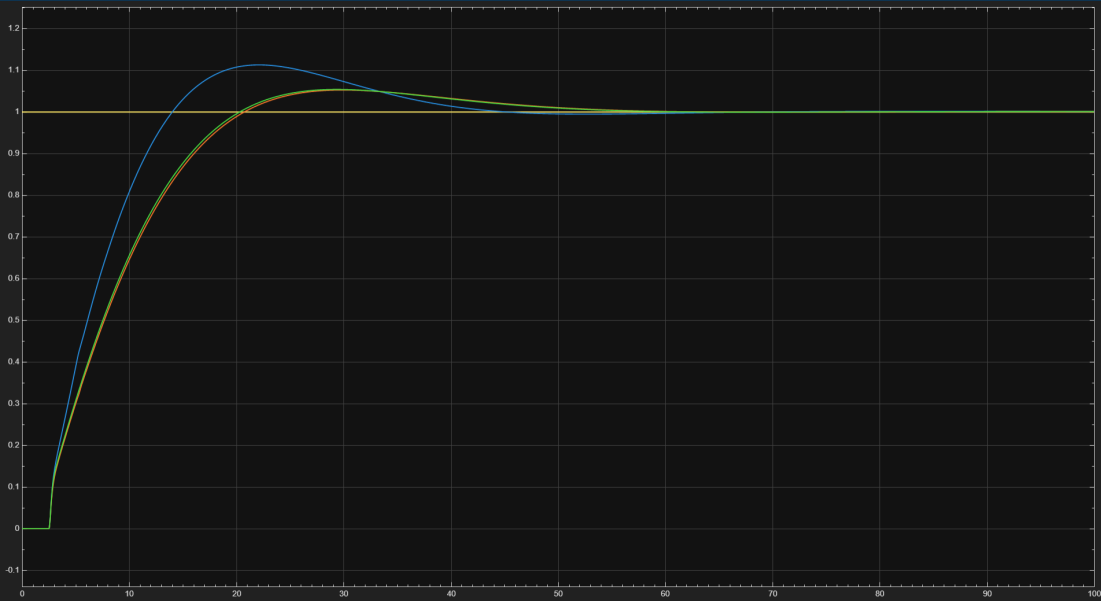
\includegraphics[width=.83\linewidth]{images/smith_comparison.png}\caption{Reported simulated responses for the controller/predictor comparison.}\label{fig:smithcompare}\end{figure}

\sechead{Validation and Interpretation}
Three evidence categories should be distinguished. First, the plant transfer function and $K_{\mathrm{DC}}=1$ are direct mathematical facts about the specified model. Second, the FOPDT/SOPDT RMSE figures are independent numerical comparisons using the parameters documented in the original analysis. Third, the relay, PID, and Smith-predictor figures originate from supplied simulation records; they do not demonstrate that all archived models have been rerun in a newly configured MATLAB/Simulink environment.

For a reproducible future comparison, use common reference trajectories, solver settings, simulation horizons, controller output limits, and disturbance scenarios. Quantitative criteria should include rise time, settling time, overshoot, control effort, and integrated absolute error,
\begin{equation}
\mathrm{IAE}=\int_{0}^{T_f}\lvert r(t)-y(t)\rvert\,dt.
\end{equation}
A model-mismatch sensitivity study should vary process gain, time constants, and transport delay separately. Such tests would support stronger robustness claims than isolated step plots alone.

\sechead{Conclusion}
This study brings together identification of delayed process dynamics, comparison of low-order models, relay-based characterization, several PID tuning approaches, and Smith prediction. The independent model comparison indicates that the reported SOPDT approximation follows the specified unit-step data slightly more closely than the FOPDT approximation. Archived controller experiments provide practical insight into tuning sensitivity and the importance of model fidelity. Repeating all PID and predictor configurations under consistent simulation conditions is the next step toward a fully quantitative controller benchmark.

\section*{Evidence and Reproducibility Note}
The source MATLAB/Simulink files and recorded figures are preserved in the associated repository. New calculations are labeled as such; previously recorded simulation figures are identified as archived evidence. This document does not claim new hardware measurements, new controller optimization, or a peer-reviewed experimental result. No personal names are included.
\end{document}
